\subsection{Results for Trajectories Estimated Using $x$ and $y$ Offset}
%\label{subsec:no_abs_results}
%\vspace{10pt}

Figure~\ref{fig:traj_no_abs_RMSE} represents the $p$-values for the Wilcoxon signed-rank test on RMSE values across $k$-fold validation datasets for the trajectories estimated using $x$ and $y$ offset in the $k$-fold testing datasets using different RNN models, and forecasting times. Darker colors in grayscale represent a higher $p$-value in a range from $0$ to $1$. The values on the secondary diagonal are all equal to $1$ and black because models equal themselves.

\begin{figure}[!ht]
	\centering
	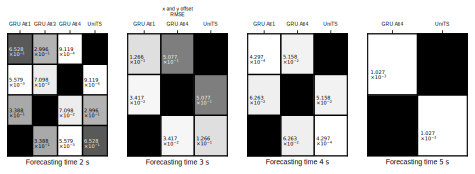
\includegraphics[width = 0.99 \linewidth]{traj_no_abs_RMSE.pdf}
	\caption{The $p$-values for the Wilcoxon signed-rank test on RMSE values across $k$-fold validation datasets for the trajectories estimated using $x$ and $y$ offset in the $k$-fold testing datasets using different RNN models, and forecasting times. Darker colors in grayscale represent a higher $p$-value in a range from $0$ to $1$. The values on the secondary diagonal are all equal to $1$ and black because models equal themselves.}
	\label{fig:traj_no_abs_RMSE}
\end{figure}

Figure~\ref{fig:wilcoxon_RMSE_traj_val_merged} contains the average RMSE across $k$-fold testing datasets using different trajectory estimation methods, validation datasets for all trajectories estimated in nested $k$-fold cross-validation by different trajectory estimation methods, RNN models, and forecasting times.

\begin{figure}[!ht]
	\centering
	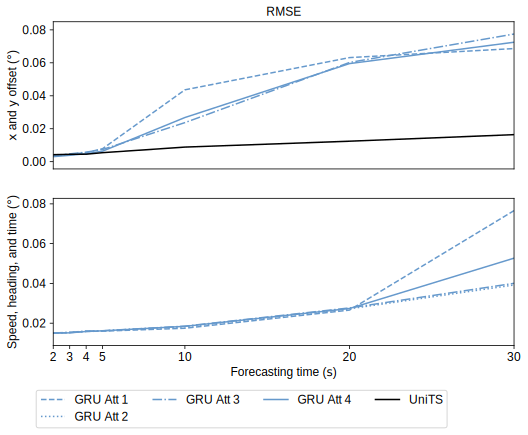
\includegraphics[width = 0.99 \linewidth]{wilcoxon_RMSE_traj_val_merged.pdf}
	\caption{The average RMSE across $k$-fold testing datasets using different trajectory estimation methods, validation datasets for all trajectories estimated in nested $k$-fold cross-validation by different trajectory estimation methods, RNN models, and forecasting times.}
	\label{fig:wilcoxon_RMSE_traj_val_merged}
\end{figure}

The average RMSE in $\degree$ ($\times 10^{-3}$), with standard deviation in brackets, across $k$-fold validation datasets for the trajectories in the $k$-fold testing datasets estimated using $x$ and $y$ offset, different RNN models, and forecasting times is listed in Table~\ref{tab:wilcoxon_no_abs_RMSE}.

\begin{table}[!ht]
	\centering
	\resizebox{\linewidth}{!}{
		\begin{tabular}{|c|c|c|c|c|c|c|c|}
			\hline
			Model & $2$ $s$ & $3$ $s$ & $4$ $s$ & $5$ $s$ & $10$ $s$ & $20$ $s$ & $30$ $s$ \\ \hline
			\multirow{2}{*}{GRU Att 1} & $3.512$ & $4.567$ & $5.475$ & $7.893$ & $43.61$ & $63.161$ & $68.645$ \\
			 & ($0.973$) & ($1.319$) & ($1.367$) & ($2.416$) & ($10.387$) & ($20.301$) & ($11.678$) \\ \hline
			\multirow{2}{*}{GRU Att 3} & $3.312$ & $4.741$ & $5.78$ & $7.406$ & $23.705$ & $60.194$ & $77.469$ \\
			 & ($0.617$) & ($0.557$) & ($1.219$) & ($1.596$) & ($11.108$) & ($40.006$) & ($39.595$) \\ \hline
			\multirow{2}{*}{GRU Att 4} & $\mathbf{3.051}$ & $\mathbf{3.864}$ & $4.858$ & $6.402$ & $26.801$ & $59.524$ & $72.495$ \\
			 & \textbf{(}$\mathbf{0.492}$\textbf{)} & \textbf{(}$\mathbf{0.506}$\textbf{)} & ($0.521$) & ($0.851$) & ($6.958$) & ($9.833$) & ($19.405$) \\ \hline
			\multirow{2}{*}{UniTS} & $4.259$ & $4.469$ & $\mathbf{4.542}$ & $\mathbf{5.471}$ & $\mathbf{8.861}$ & $\mathbf{12.431}$ & $\mathbf{16.414}$ \\
			 & ($3.507$) & ($2.909$) & \textbf{(}$\mathbf{0.66}$\textbf{)} & \textbf{(}$\mathbf{0.975}$\textbf{)} & \textbf{(}$\mathbf{1.366}$\textbf{)} & \textbf{(}$\mathbf{1.552}$\textbf{)} & \textbf{(}$\mathbf{2.472}$\textbf{)} \\ \hline
		\end{tabular}
	}
	\caption{The average RMSE in $\degree$ ($\times 10^{-3}$), with standard deviation in brackets, across $k$-fold validation datasets for the trajectories in the $k$-fold testing datasets estimated using $x$ and $y$ offset, different RNN models, and forecasting times.}
	\label{tab:wilcoxon_no_abs_RMSE}
\end{table}

The GRU Att 4 model achieved the lowest RMSE for trajectories estimated using $x$ and $y$ offset, and a forecasting time of $2$, and $3$ $s$ with average values and standard deviation (in brackets) that equal $3.05 \times 10^{-3}$ $\degree$ ($0.49 \times 10^{-3}$ $\degree$), and $3.86 \times 10^{-3}$ $\degree$ ($0.51 \times 10^{-3}$ $\degree$) respectively.

The GRU Att 4 model does not have a statistically significantly different RMSE than the GRU Att 1, GRU Att 3, and UniTS models for $x$ and $y$ offset using a forecasting time of $2$ $s$, with $p$-values equaling $5.579 \times 10^{-3}$, $7.098 \times 10^{-2}$, and $9.119 \times 10^{-4}$.

\markertable{tab:\label{tab:RMSE:no:abs:p:2}}

The GRU Att 4 model does not have a statistically significantly different RMSE than the GRU Att 1, and UniTS models for $x$ and $y$ offset using a forecasting time of $3$ $s$, with $p$-values equaling $3.417 \times 10^{-2}$, and $5.077 \times 10^{-1}$.

\markertable{tab:\label{tab:RMSE:no:abs:p:3}}

The UniTS model achieved the lowest RMSE for trajectories estimated using $x$ and $y$ offset, and a forecasting time of $4$, $5$, $10$, $20$, and $30$ $s$ with average values and standard deviation (in brackets) that equal $4.54 \times 10^{-3}$ $\degree$ ($0.66 \times 10^{-3}$ $\degree$), $5.47 \times 10^{-3}$ $\degree$ ($0.97 \times 10^{-3}$ $\degree$), $8.86 \times 10^{-3}$ $\degree$ ($1.37 \times 10^{-3}$ $\degree$), $12.43 \times 10^{-3}$ $\degree$ ($1.55 \times 10^{-3}$ $\degree$), and $16.41 \times 10^{-3}$ $\degree$ ($2.47 \times 10^{-3}$ $\degree$) respectively.

The UniTS model does not have a statistically significantly different RMSE than the GRU Att 1, and GRU Att 4 models for $x$ and $y$ offset using a forecasting time of $4$ $s$, with $p$-values equaling $4.297 \times 10^{-4}$, and $5.158 \times 10^{-2}$.

\markertable{tab:\label{tab:RMSE:no:abs:p:4}}

The UniTS model does not have a statistically significantly different RMSE than the GRU Att 4 model for $x$ and $y$ offset using a forecasting time of $5$ $s$, with a $p$-value equaling $1.027 \times 10^{-3}$.

\markertable{tab:\label{tab:RMSE:no:abs:p:5}}

